%!TEX root = TTK4215-Summary.tex
\section{Extremum seeking}
The basic idea: Want to find the optimal plant input $\theta^*$ that maximises the output $y$. Add a slow periodic perturbation to our estimate $\hat{\theta}$. If increasing $\theta$ increases $y$, then $y$ will oscillate in phase with $\theta$. In the opposite case, $y$ with be out of phase with $\theta$. The DC component of $y$ is removed with a high-pass filter, and the result multiplied with the perturbation signal. The product will have a positive DC component if $y$ and $\theta$ are in phase, and negative DC if they are out of phase. This DC component is extracted with a low-pass filter, and is then a value indicating how far off $\theta$ is, and in what direction. This is integrated and multiplied with a gain $k$ to form the estimate $\hat{\theta}$. Pretty clever.

\begin{figure}[htbp]
\begin{center}
	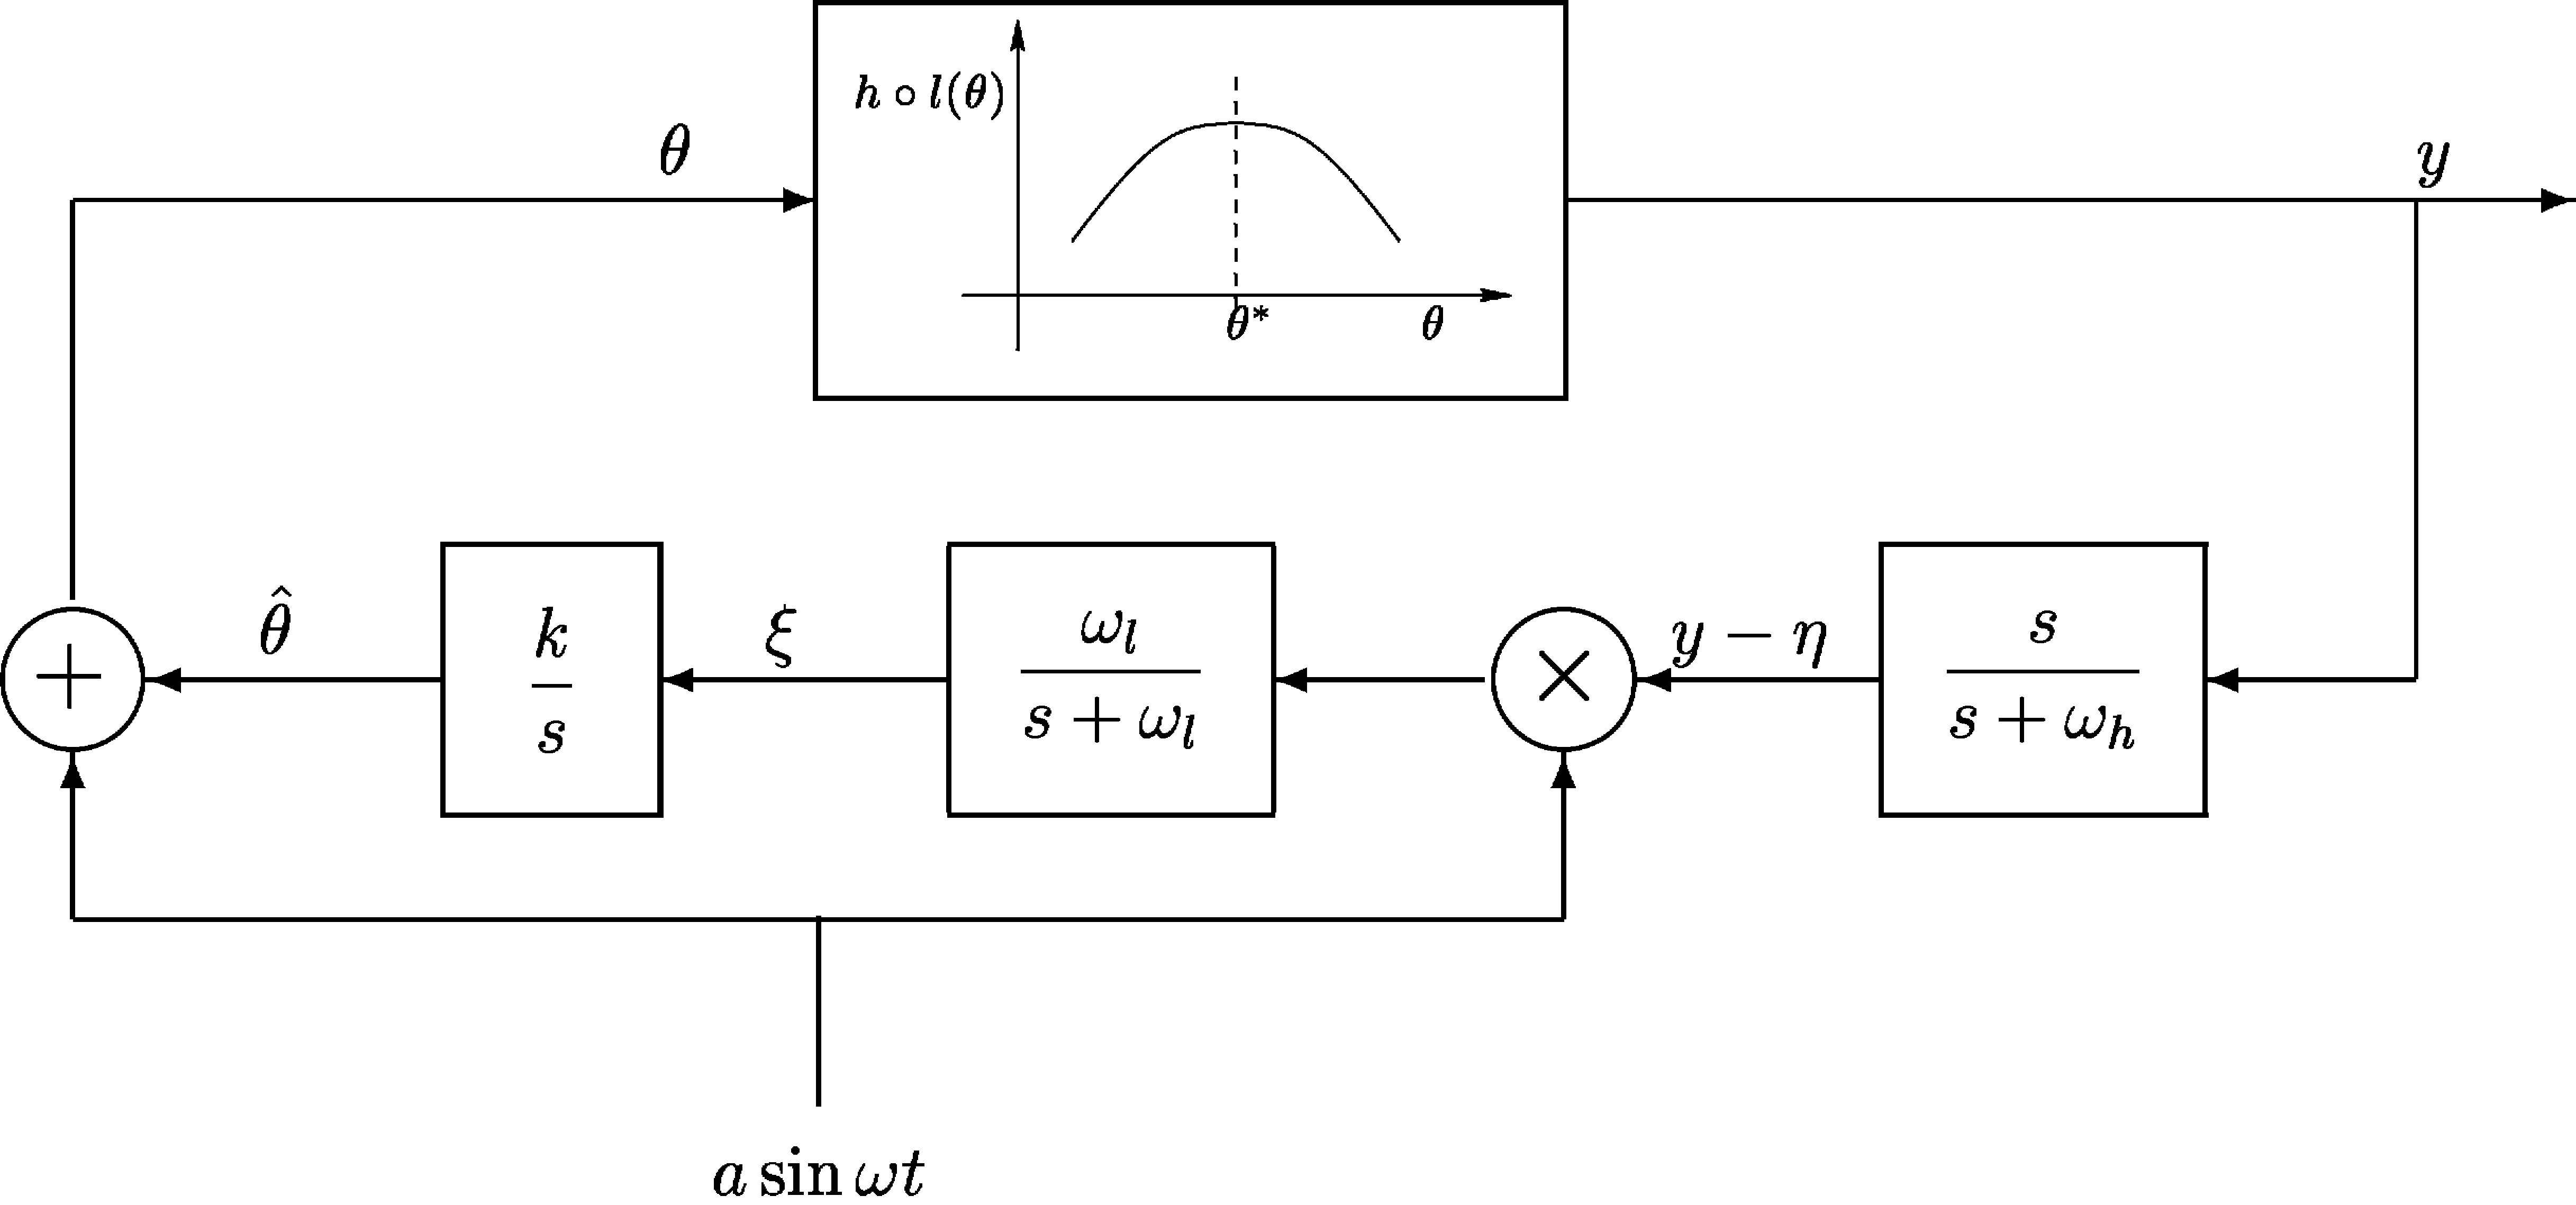
\includegraphics[width = \textwidth]{extremum-seeking}
	\caption{Block diagram for extremum seeking}
	\label{fig:MRAC}
\end{center}
\end{figure}